\documentclass{article}

\usepackage{amsthm}
\usepackage{amsfonts}
\usepackage{amsmath}
\usepackage{amssymb}
\usepackage{fullpage}
\usepackage{geometry}
\geometry{margin=1.3in}


\usepackage{graphicx}

\usepackage[usenames]{color}
\usepackage{hyperref}
  \hypersetup{
    colorlinks = true,
    urlcolor = blue,       % color of external links using \href
    linkcolor= blue,       % color of internal links 
    citecolor= blue,       % color of links to bibliography
    filecolor= blue,        % color of file links
    }
    
\usepackage{listings}

\definecolor{dkgreen}{rgb}{0,0.6,0}
\definecolor{gray}{rgb}{0.5,0.5,0.5}
\definecolor{mauve}{rgb}{0.58,0,0.82}

\lstset{frame=tb,
  language=haskell,
  aboveskip=3mm,
  belowskip=3mm,
  showstringspaces=false,
  columns=flexible,
  basicstyle={\small\ttfamily},
  numbers=none,
  numberstyle=\tiny\color{gray},
  keywordstyle=\color{blue},
  commentstyle=\color{dkgreen},
  stringstyle=\color{mauve},
  breaklines=true,
  breakatwhitespace=true,
  tabsize=3
}

\theoremstyle{theorem} 
   \newtheorem{theorem}{Theorem}[section]
   \newtheorem{corollary}[theorem]{Corollary}
   \newtheorem{lemma}[theorem]{Lemma}
   \newtheorem{proposition}[theorem]{Proposition}
\theoremstyle{definition}
   \newtheorem{definition}[theorem]{Definition}
   \newtheorem{example}[theorem]{Example}
\theoremstyle{remark}    
  \newtheorem{remark}[theorem]{Remark}


\title{CPSC 406}
\author{Tyler Lewis  \\ Chapman University}

\date{\today}

\begin{document}

\maketitle

\tableofcontents

\section{Homework}\label{intro}
\subsection{HW 1}

\begin{minipage}{0.4\textwidth}
\begin{itemize}
\item[\textbf{\emph{NFA2DFA}}] In order to convert the provided NFA to DFA I considered each possible combination of P, Q, R, and S, and considered each possible combination its own state. The included figure details every possible state the NFA/DFA may find itself in.
\end{itemize}
\end{minipage}%
%
\begin{minipage}{0.4\textwidth}
\begin{center}
    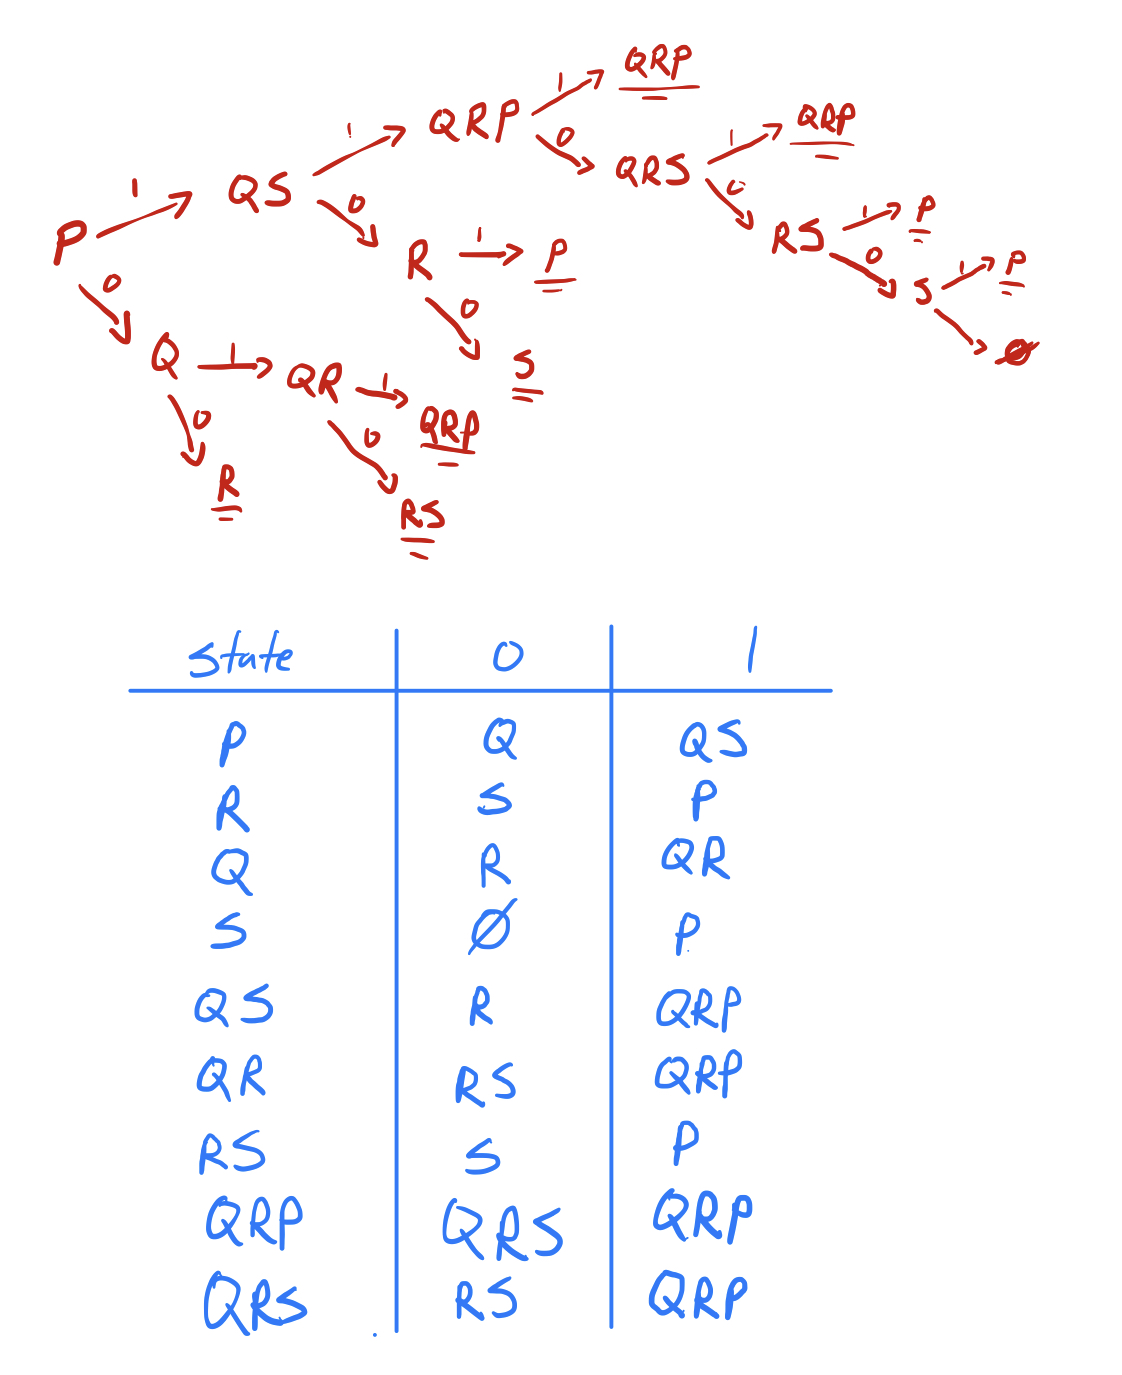
\includegraphics[width=\textwidth]{hw1.jpg}
    % \captionof{figure}{Gripper}
    \label{img:g}
\end{center}
\end{minipage}

\subsection{HW 3}

{\bf Question 1:}

    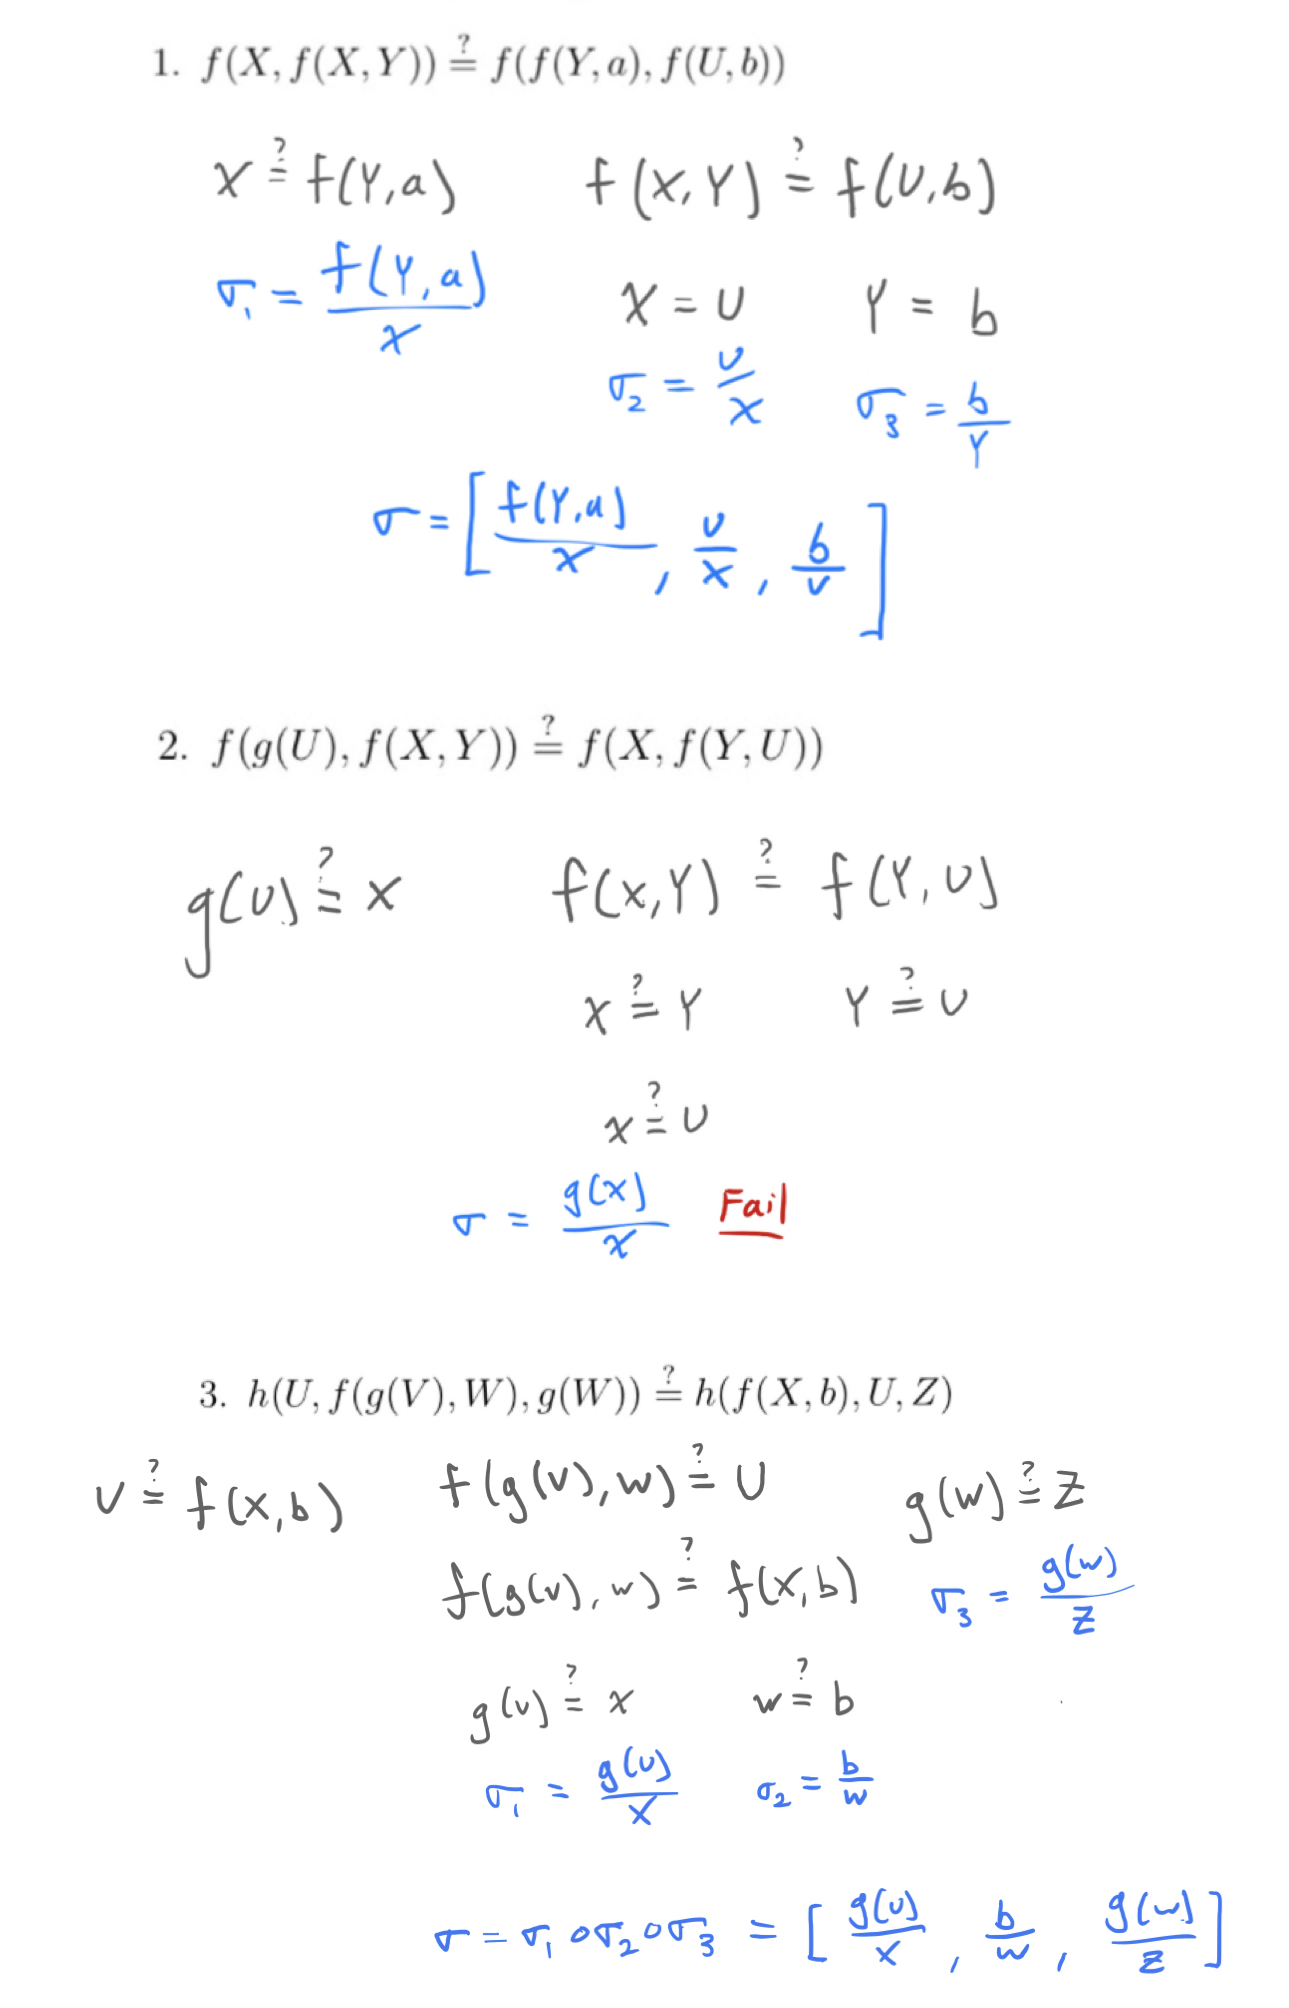
\includegraphics[width=10cm]{hw3q1.jpg}
    
% \end{center}
% \end{minipage}

{\bf Question 2:}
\begin{verbatim}
    ?- twoway(W,a)
    
    ?- conn(W,a), conn(a,W)
    
    ?- addr(W,a), addr(a,Z), serv(Z), addr(Z,W)
\end{verbatim}

\subsection{HW 6}
\href{https://hackmd.io/@alexhkurz/ByaOUajy2}{HackMD Page}

    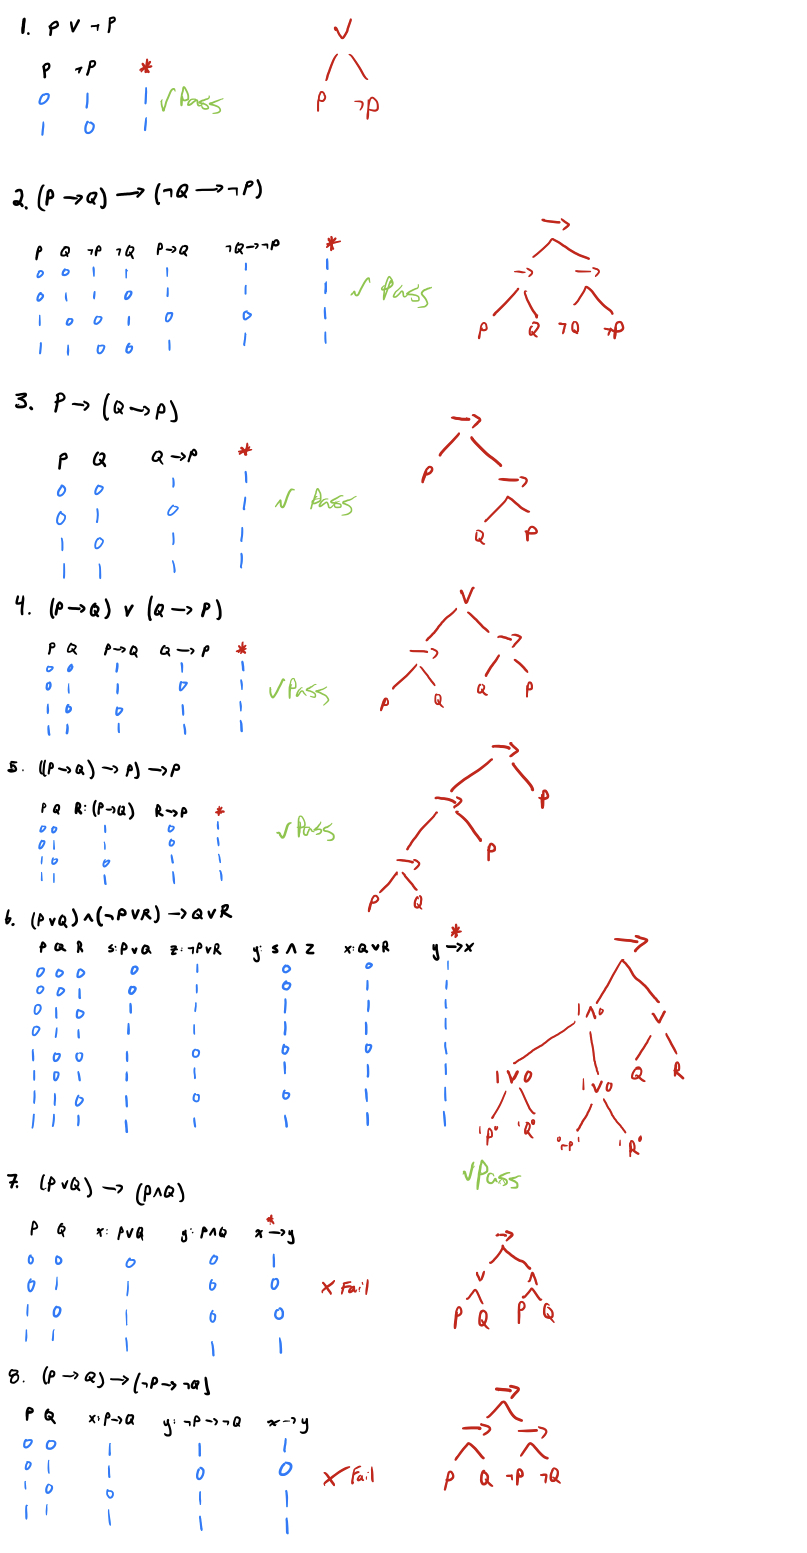
\includegraphics[width=9cm]{hw6.jpg}

\subsection{HW 9}

\href{https://github.com/alexhkurz/algorithm-analysis-2023/blob/main/resources/model-checking/Needham-Schroeder.md}{Assignment Brief}
\\

{\bf Exercise 1:}

\begin{itemize}
\item `success`: This is a propositional variable that is true if both statusA and statusB are ok. This variable is used to check whether the protocol was executed successfully.
\item `aliceBob`: This is a propositional variable that is true if `partnerA` is `bob`. This variable is used to check whether Alice successfully communicated with Bob.

\item `bobAlice`: This is a propositional variable that is true if `partnerB` is `alice`. This variable is used to check whether Bob successfully communicated with Alice.

\item `\&\&`: This is the logical AND operator. It is used to combine two boolean expressions and evaluate to true if both expressions are true.

\item `$\rightarrow$`: This is the implication operator. It is used to specify a condition that must be satisfied in order for an action to occur. For example, in the statement `(data.key == keyA) \&\& (data.d1 == nonceA) $\rightarrow$`, the action on the right-hand side can only occur if the conditions on the left-hand side are true.

\item `[]`: This is the "always" operator. It is used to specify a condition that must always be true in order for a property to hold. For example, the property $[] (success \rightarrow (aliceBob \land bobAlice))$ specifies that if the protocol was executed successfully, then Alice must have communicated with Bob and Bob must have communicated with Alice.

\item `[]A`: This is the "always eventually" operator. It is used to specify a condition that must eventually be true in order for a property to hold.

\end{itemize}


{\bf Exercise 2:}

The first formula, 'ltl {[] (success \&\& aliceBob -> bobAlice)} is not violated', is verified as correct, meaning that the property holds for all possible executions of the protocol. However, the second formula, 'ltl {[] (success \&\& bobAlice -> aliceBob)} is violated', is not correct, meaning that there exists at least one execution of the protocol where the property does not hold.


{\bf Exercise 3:}

The property that is violated produces an execution sequence where the specified property does not hold. Based on the trail file, the length of the execution sequence that violated the property is 84 steps. This is the total number of steps taken during the execution of the protocol before the assertion was violated.

{\bf Exercise 4:}

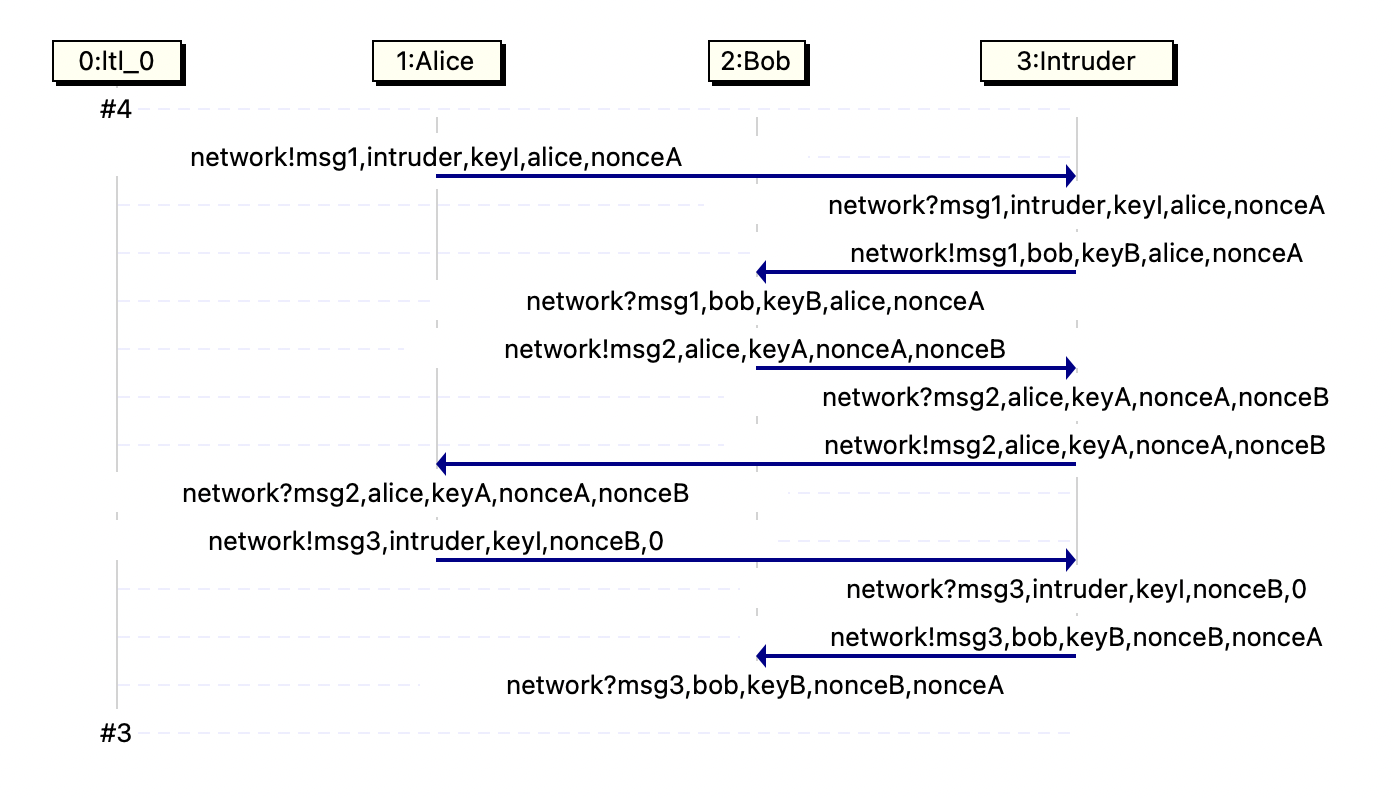
\includegraphics[width=10cm]{hw9.png}
The attack was successful because the intruder was able to intercept the messages exchanged between Alice and Bob and alter them in such a way that Bob believed she was communicating with Alice when in fact he was communicating with the intruder. Specifically, the intruder was able to send messages to Bob and sign them with Alice's key, thereby convincing Bob that he was receiving messages from Alice when in fact they were coming from the intruder.

\subsection{HW 11}
\subsubsection{L11.1}
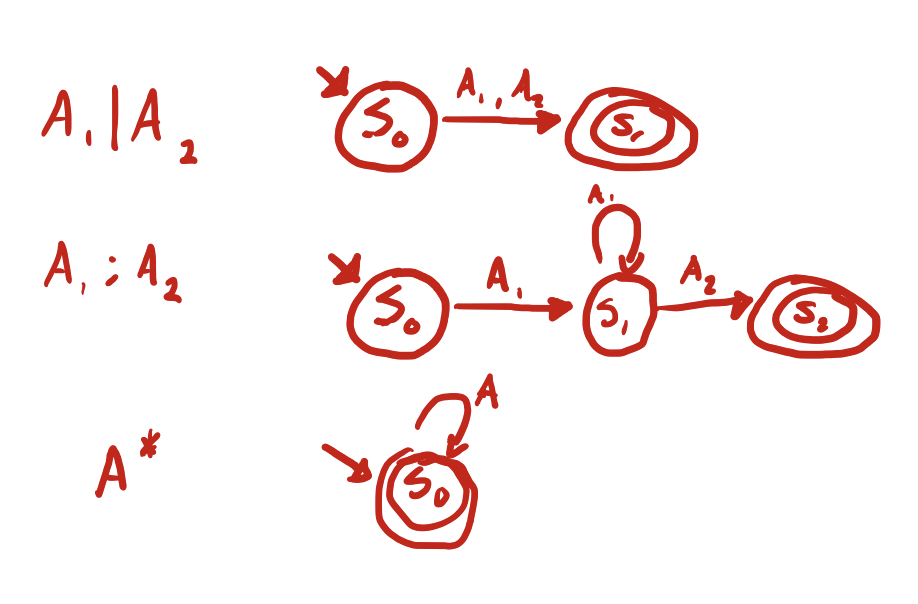
\includegraphics[width=10cm]{hw11-2.jpeg}

\subsubsection{L11.2}

a) The set of strings over alphabet {0, 1,...,9}  such that the final digit has appeared before.
\\\\
The regular expression which I think may satisfy this (simplified) is as follows, with S being any of the set of characters in our alphabet, and N being a specific character
\[S*NS*N\]
b) The set of strings consisting of zero or more a's followed by zero or more b's, followed by zero or more c's.
\[A*B*C*\]
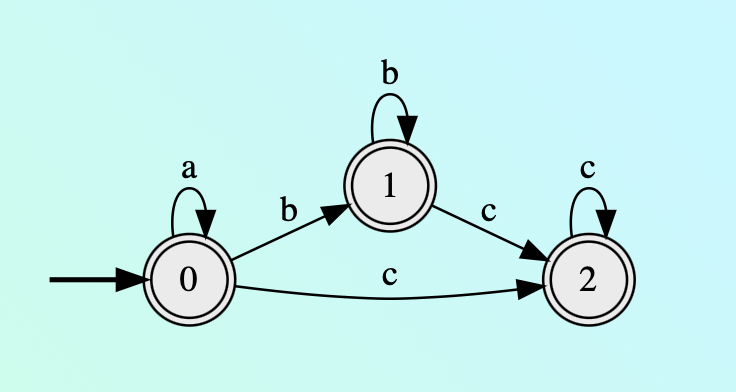
\includegraphics[width = 10cm]{hw11-1.png}

\subsection{HW 12}

\href{https://hackmd.io/@alexhkurz/ryEdSuVXh}{HackMD Page}\\
\begin{itemize}
    \item[Exercise 1:] \textit{Have a look at peterson.py. What program behavior do you expect? Is your expectation confirmed when you run the program?}
    
    peterson.py uses a busy waiting lock, my expectation that this is adequate to ensure a result of 20,000 is confirmed by running the program

    \item[Exercise 2:] \textit{Analyse the Java program peterson in the same way as you analysed the Python program in the previous exercise. Make sure to run the Java program on your local machine. What observations do you make?}

    peterson in Java follows the same busy waiting lock scheme as in the python code.

    \item[Exercise 3:] \textit{Explain why the outcome
    a = 0, b = 0
    is not sequentially consistent, but the other three outcomes are.}
    
    The way the program is written, this outcome would only arise if one of the threads failed or the order of operations was modified within the threads. Assuming the threads execute synchronously, and memory is properly shared between threads, then x and/or y will always be set to 1 before the assignment of a and/or b. 

    \item[Exercise 4:] \textit{Report the results you get from running memoryModelWithStats on your local machine. Include the specs of our processor, in particular the number of cores. If you can find out something about the cashes, add this as well.}
\begin{verbatim}
    Outcomes after 1000 iterations:
    (0, 0): 4
    (0, 1): 487
    (1, 0): 509https://www.overleaf.com/project/63f2ff20adaf2530bdc3f4fa
    (1, 1): 0
\end{verbatim}

\begin{verbatim}
    Hardware Overview:

      Model Name: MacBook Pro
      Chip: Apple M2 Pro
      Total Number of Cores: 12 (8 performance and 4 efficiency)
      Memory: 32 GB
\end{verbatim}
    

    \item[Exercise 5:] \textit{You can force sequential consistency of memoryModelWithStats by declaring certain variables volatile. In general, declaring variables as volatile comes at cost in execution time, so we want to use this sparingly. Which variables must be declare as volatile to ensure sequential consistency? Measure and report the effect that volatile has on your run time (I use java Main | gnomon).}

    Declaring variables (x, y, a, and b) as volatile will achieve sequential consistency. 

    I was unable to get gnomon running but chatGPT indicates this may come at a cost in execution time, as accesses to volatile variables may be slower than non-volatile variables.



\end{itemize}

\section{Creative Paper}
\subsection{Introduction}

\textbf{THE YEAR IS 2048.}

The world finds itself under the control of a single global regime, which, citing national security and unity, has imposed harsh restrictions on the World Wide Web, forever altering the digital communication landscape. Privacy has become a relic of the past. \textbf{This oppressive regime is embodied in AI-Titan, a government-affiliated entity formed by the consolidation of tech giants and absorbed into the government due to increased regulations and the addition of AI to every aspect of their function.}

AI-Titan now owns all data centers and acts as the authority responsible for issuing \textbf{identity encryption keys necessary for internet access.} Without these keys, the internet becomes inaccessible, leaving users disconnected from the digital realm. The regime has banned the use of third-party encryption, requiring individuals to encrypt their data with their personal private key or transmit it in plaintext, allowing the regime to monitor and control information at will.

The regime's influence extends to cloud computing, where AI-Titan has become the sole provider of cloud services. With control over DNS and Certificate Authority (CA) systems, AI-Titan establishes a complete monopoly over the public internet. Every website and data flow falls under their jurisdiction, solidifying the regime's grip on information and further eroding privacy.

Under the regime's control, the Domain Name System (DNS), once a neutral phonebook of the internet, is a tool of surveillance and censorship. DNS servers, now under the regime's command, remove websites deemed undesirable from their records, effectively erasing them from the digital world. All communication infrastructure is owned by the regime \textbf{and is monitored closely by AI-Titan.}

\subsection{A Glimmer of Hope}

\textbf{A glimmer of hope emerges amidst the digital darkness.} A movement, known as the Digital Liberation Front (DiLF), emerges with the aim of restoring privacy, freedom, and autonomy in the digital realm.

Recognizing the regime's inability to control satellite networks orbiting Earth, the DiLF proposes a daring solution: a new distributed satellite internet that bypasses the regime's infrastructure.

Their ambitious plan involves re-purposing the existing satellite network, which was put there during the space race bubble in the 20s and 30s. The DiLF establishes SatNet: a massive distributed system running on tens of thousands of satellites. The network uses advanced consensus algorithms and an AI governance model to create a decentralized, peer-to-peer network accessible through low-power ground terminal stations. This not only undermines the harsh internet surveillance of the regime but marks a revolution of the World Wide Web.

\subsection{The Creation of SatNet}

SatNet becomes a platform where information flows freely, shielded by anonymity and distribution. Communications remain encrypted and untraceable. However, the DiLF recognizes that to maintain trust and security, SatNet requires a robust AI governance model that operates autonomously, ensuring a reliable and resilient flow of information without the need for human intervention, which has proven problematic in every failure of the human race.

To achieve this, SatNet incorporates an innovative AI governance system called Autonomous Consensus Control (ACC). ACC is a self-learning, self-improving AI system designed to manage SatNet's operations, consensus protocols, and identity system.

At the core of SatNet's ACC is the Identity Enhancement Protocol (IEP). The IEP allows individuals to participate in the consensus process and contribute to the network's improvement over time. Users are assigned unique digital identities that are securely stored within SatNet's distributed ledger. These identities serve as the foundation for trust and governance within the network.

The IEP utilizes advanced cryptographic techniques, such as zero-knowledge proofs an encryption, to protect the privacy and integrity of user identities. Users can securely authenticate their identities and participate in consensus without revealing sensitive personal information. This ensures that individuals can engage in the governance process without fear of surveillance or manipulation by external entities.

Within SatNet's AI governance model, the consensus process is facilitated by a sophisticated AI algorithm called Decentralized Consensus Coordinator (DCC). The DCC is responsible for coordinating the consensus among validating nodes, ensuring that the majority of nodes agree on the order and validity of transactions and information within the network.

The DCC employs a hybrid consensus mechanism that combines proof-of-stake (PoS) and proof-of-reputation (PoR) algorithms. Validating nodes, including both trusted satellites and participating ground stations, stake their resources and reputation to earn the right to validate and propose new blocks of transactions. This consensus mechanism ensures that the network remains secure, efficient, and resistant to attacks, while also preventing concentration of power in a single entity.

To continuously improve the network's performance and resilience, SatNet incorporates a feedback loop mechanism called Adaptive Network Optimization (ANO). ANO leverages machine learning algorithms to analyze network performance metrics, identify bottlenecks or vulnerabilities, and dynamically optimize the routing and resource allocation within SatNet. This self-optimizing capability allows the network to adapt and evolve over time, enhancing its efficiency and resistance to potential threats.

In addition to the AI governance model, SatNet embraces transparency and inclusivity through its Decentralized Governance Forum (DGF). The DGF serves as an open platform where stakeholders, including users, developers, and satellite operators, can propose and discuss improvements, changes, and policies related to SatNet's operation. Through a decentralized voting mechanism, decisions regarding network upgrades, protocol changes, and governance rules are collectively determined by the community, ensuring a fair and democratic approach to network governance.

As SatNet matures, its AI governance model not only ensures the network's integrity and security but also facilitates continuous innovation and improvement. With the participation of individuals from diverse backgrounds, SatNet becomes a collaborative ecosystem where ideas thrive and the network's capabilities expand.

\subsection{A New Era of Digital Freedom}

With the deployment of SatNet and its advanced AI governance model, the DiLF movement gains significant traction worldwide. People from all walks of life join the cause, driven by the desire for privacy, freedom, and autonomy in the digital realm.

SatNet's distributed satellite internet gradually outshines the regime-controlled internet, attracting a growing user base seeking an alternative to the oppressive surveillance regime. The network becomes a powerful symbol of resistance, resilience, and human ingenuity.

As more individuals join SatNet, the network's decentralized nature and AI governance model allow it to scale and adapt effortlessly. SatNet becomes a catalyst for positive change, empowering individuals to reclaim control over their digital lives. People communicate freely, share knowledge, and collaborate across borders, fostering innovation, cultural exchange, and social progress.

Governments, witnessing the transformative impact of SatNet and the demands of their own citizens, begin to reassess their approach to digital governance. Inspired by the success of the DiLF movement, they gradually dismantle the regimes own surveillance apparatus, embracing principles of decentralization, privacy, and individual rights.

In this new era of digital freedom, SatNet continues to evolve and improve. The network becomes a global cooperative effort, with nations and organizations collaborating to expand its coverage, enhance its capabilities, and ensure its long-term sustainability.

The story of SatNet and its AI governance model stands as a testament to the indomitable spirit of humanity and its quest for freedom. It reminds us that even in the face of oppressive regimes and technological challenges, innovation, resilience, and collective action can pave the way for a brighter and more inclusive digital future.

\subsection{Technical Analysis}

SatNet, as envisioned in the year 2048, represents a distributed satellite internet system developed by the Digital Liberation Front (DiLF) to counter the oppressive regime's control over the global internet infrastructure. This technical analysis explores the key components and technologies that underpin SatNet and its advanced AI governance model, which empower individuals with privacy, freedom, and autonomy in the digital realm.

\begin{itemize}
\item Network Architecture:
\begin{itemize}
\item SatNet's network architecture utilizes repurposed satellites from the existing satellite network, forming a distributed system accessible through low-power ground terminal stations.
\item Autonomous Consensus Control (ACC) manages SatNet's operations, consensus protocols, and identity system, ensuring trust, security, and autonomy within the network. ACC incorporates artificial intelligence techniques, such as machine learning, reinforcement learning, and distributed decision-making algorithms.
\item The Identity Enhancement Protocol (IEP) enables individuals to participate in the consensus process and contribute to network improvement. Users are assigned unique digital identities stored within SatNet's distributed ledger, with advanced cryptographic techniques protecting privacy and integrity.
\item The Decentralized Consensus Coordinator (DCC) facilitates consensus among validating nodes using a hybrid proof-of-stake (PoS) and proof-of-reputation (PoR) algorithm.
\item Adaptive Network Optimization (ANO) uses machine learning algorithms to analyze network performance, optimize routing and resource allocation, and enhance the network's efficiency and resilience.
\item The Decentralized Governance Forum (DGF) provides an open platform for stakeholders to propose and discuss improvements, with decisions made through decentralized voting.
\end{itemize}

\item Proof-of-Stake (PoS) and Proof-of-Reputation (PoR) Algorithms:
\begin{itemize}
\item PoS and PoR are consensus algorithms used in some blockchain networks today. PoS allows validators to secure the network and create new blocks based on the number of coins they hold and stake. PoR is a reputation-based algorithm where validators' past behavior and reputation influence their role in the consensus process.
\end{itemize}

\item Zero-Knowledge Proofs:
\begin{itemize}
\item Zero-knowledge proofs are cryptographic protocols that allow a party to prove the validity of a statement without revealing any additional information. SatNet utilizes zero-knowledge proofs to protect privacy and integrity within its identity system.
\end{itemize}

\item Advanced Cryptographic Encryption:
\begin{itemize}
\item SatNet employs advanced cryptographic encryption techniques, including asymmetric (public-key) encryption, symmetric encryption, and hashing algorithms, ensuring the privacy and security of user identities and communications within the network.
\end{itemize}

\item Machine Learning Algorithms for Adaptive Network Optimization (ANO):
\begin{itemize}
\item ANO in SatNet utilizes machine learning algorithms to analyze network performance metrics, identify bottlenecks or vulnerabilities, and optimize routing and resource allocation, enhancing the network's efficiency and resilience.
\end{itemize}

\item Autonomous Consensus Control (ACC):
\begin{itemize}
\item ACC is an AI governance system designed to manage SatNet's operations, consensus protocols, and identity system. It ensures the network's autonomy, security, and reliability without detailed specifications of its exact implementation.
\end{itemize}
\end{itemize}

\subsection{Conclusion}

The collapse of the traditional internet led to a new internet emerging from the grassroots, powered by a wide range of algorithms. This new internet has the potential to replace the old internet and brings about significant societal changes. The regimes infiltration of the internet disrupted communication channels and challenged the power dynamics with the people. However, the DiLFs and their efforts to give rise to a new internet empowered individuals and communities, providing greater control and autonomy over digital experiences like nobody had ever seen before on such a large scale.

The impact of the new internet on society is profound. Individuals now connect their devices through networks that prioritize decentralized and peer-to-peer connections. This shift allows for greater inclusivity, collaboration, and shared interests among communities. The new internet challenged the centralized control of the regime and won. SatNet provided an avenue of enhanced privacy and security through encryption and data protection algorithms, with an impenetrable satellite-enabled physical layer.

Societal developments and advancements in algorithms are closely intertwined. In this fictional story, societal demands for autonomy, privacy, and control drove the development of algorithms that prioritize user empowerment and decentralized networks. Societal demands will shape the future digital landscape, and hopefully one that is more participatory, resilient, and in line with individual needs than the needs and desires of those in control.


\begin{thebibliography}{99}
\bibitem[ALG]{Alg} \href{https://github.com/alexhkurz/algorithm-analysis-2023}{Algorithm Analysis}, Chapman University, 2023.
\end{thebibliography}

\end{document}